%\documentclass[11pt,twoside]{mitthesis}
%\usepackage{tikz}
%\usepackage{circuitikz}
%\usepackage{amsmath}
%\usepackage{float}
%\newcommand{\ohm}{$\Omega$ }
%\begin{document}
\chapter{Firmware}

The firmware is structured in three sections - USB data reception and transmission, DAC operation, and ADC operation.

Libopencm3, licensed under the GNU LGPL v3, is used extensively in this firmware.

Block Diagram

\section{ADC}
The ADCS7476 is a successive approximation ADC with an SPI interface.  
In operation, a master device initiates a conversion by pulling $\overline{\mbox{\texttt{CS}}}$ low, then clocks in data using the \texttt{CK} line and reading \texttt{SDATA}.

\begin{figure}[H]
	\label{fig:adc-timing}
  \begin{center}
      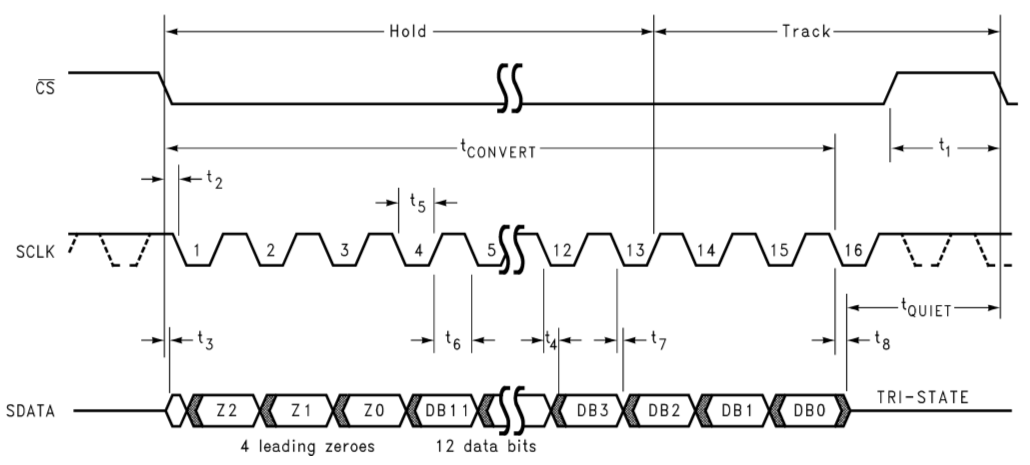
\includegraphics[width=\textwidth]{../adc-timing.png}
      \caption{ADCS7476 Serial Interface Timing Diagram}
  \end{center}
\end{figure}

The ADC firmware configures two 32-bit timers and the DMA to record data from up to sixteen external ADCs.
The two timers are responsible for driving the Chip Select and Clock lines on all of the ADCs.
The timing of the Chip Select line determines the sampling frequency and the Clock line is driven at the ADCS7476's maximum clock frequency of 20MHz.
On the rising edge of each clock cycle, the DMA is triggered to sample the data lines of each ADC.
A trigger causes the DMA to store each of the 16 pin states on \texttt{PORT E} as a 16-bit integer in the buffer \texttt{datas}.

\begin{figure}[H]
  \begin{center}
      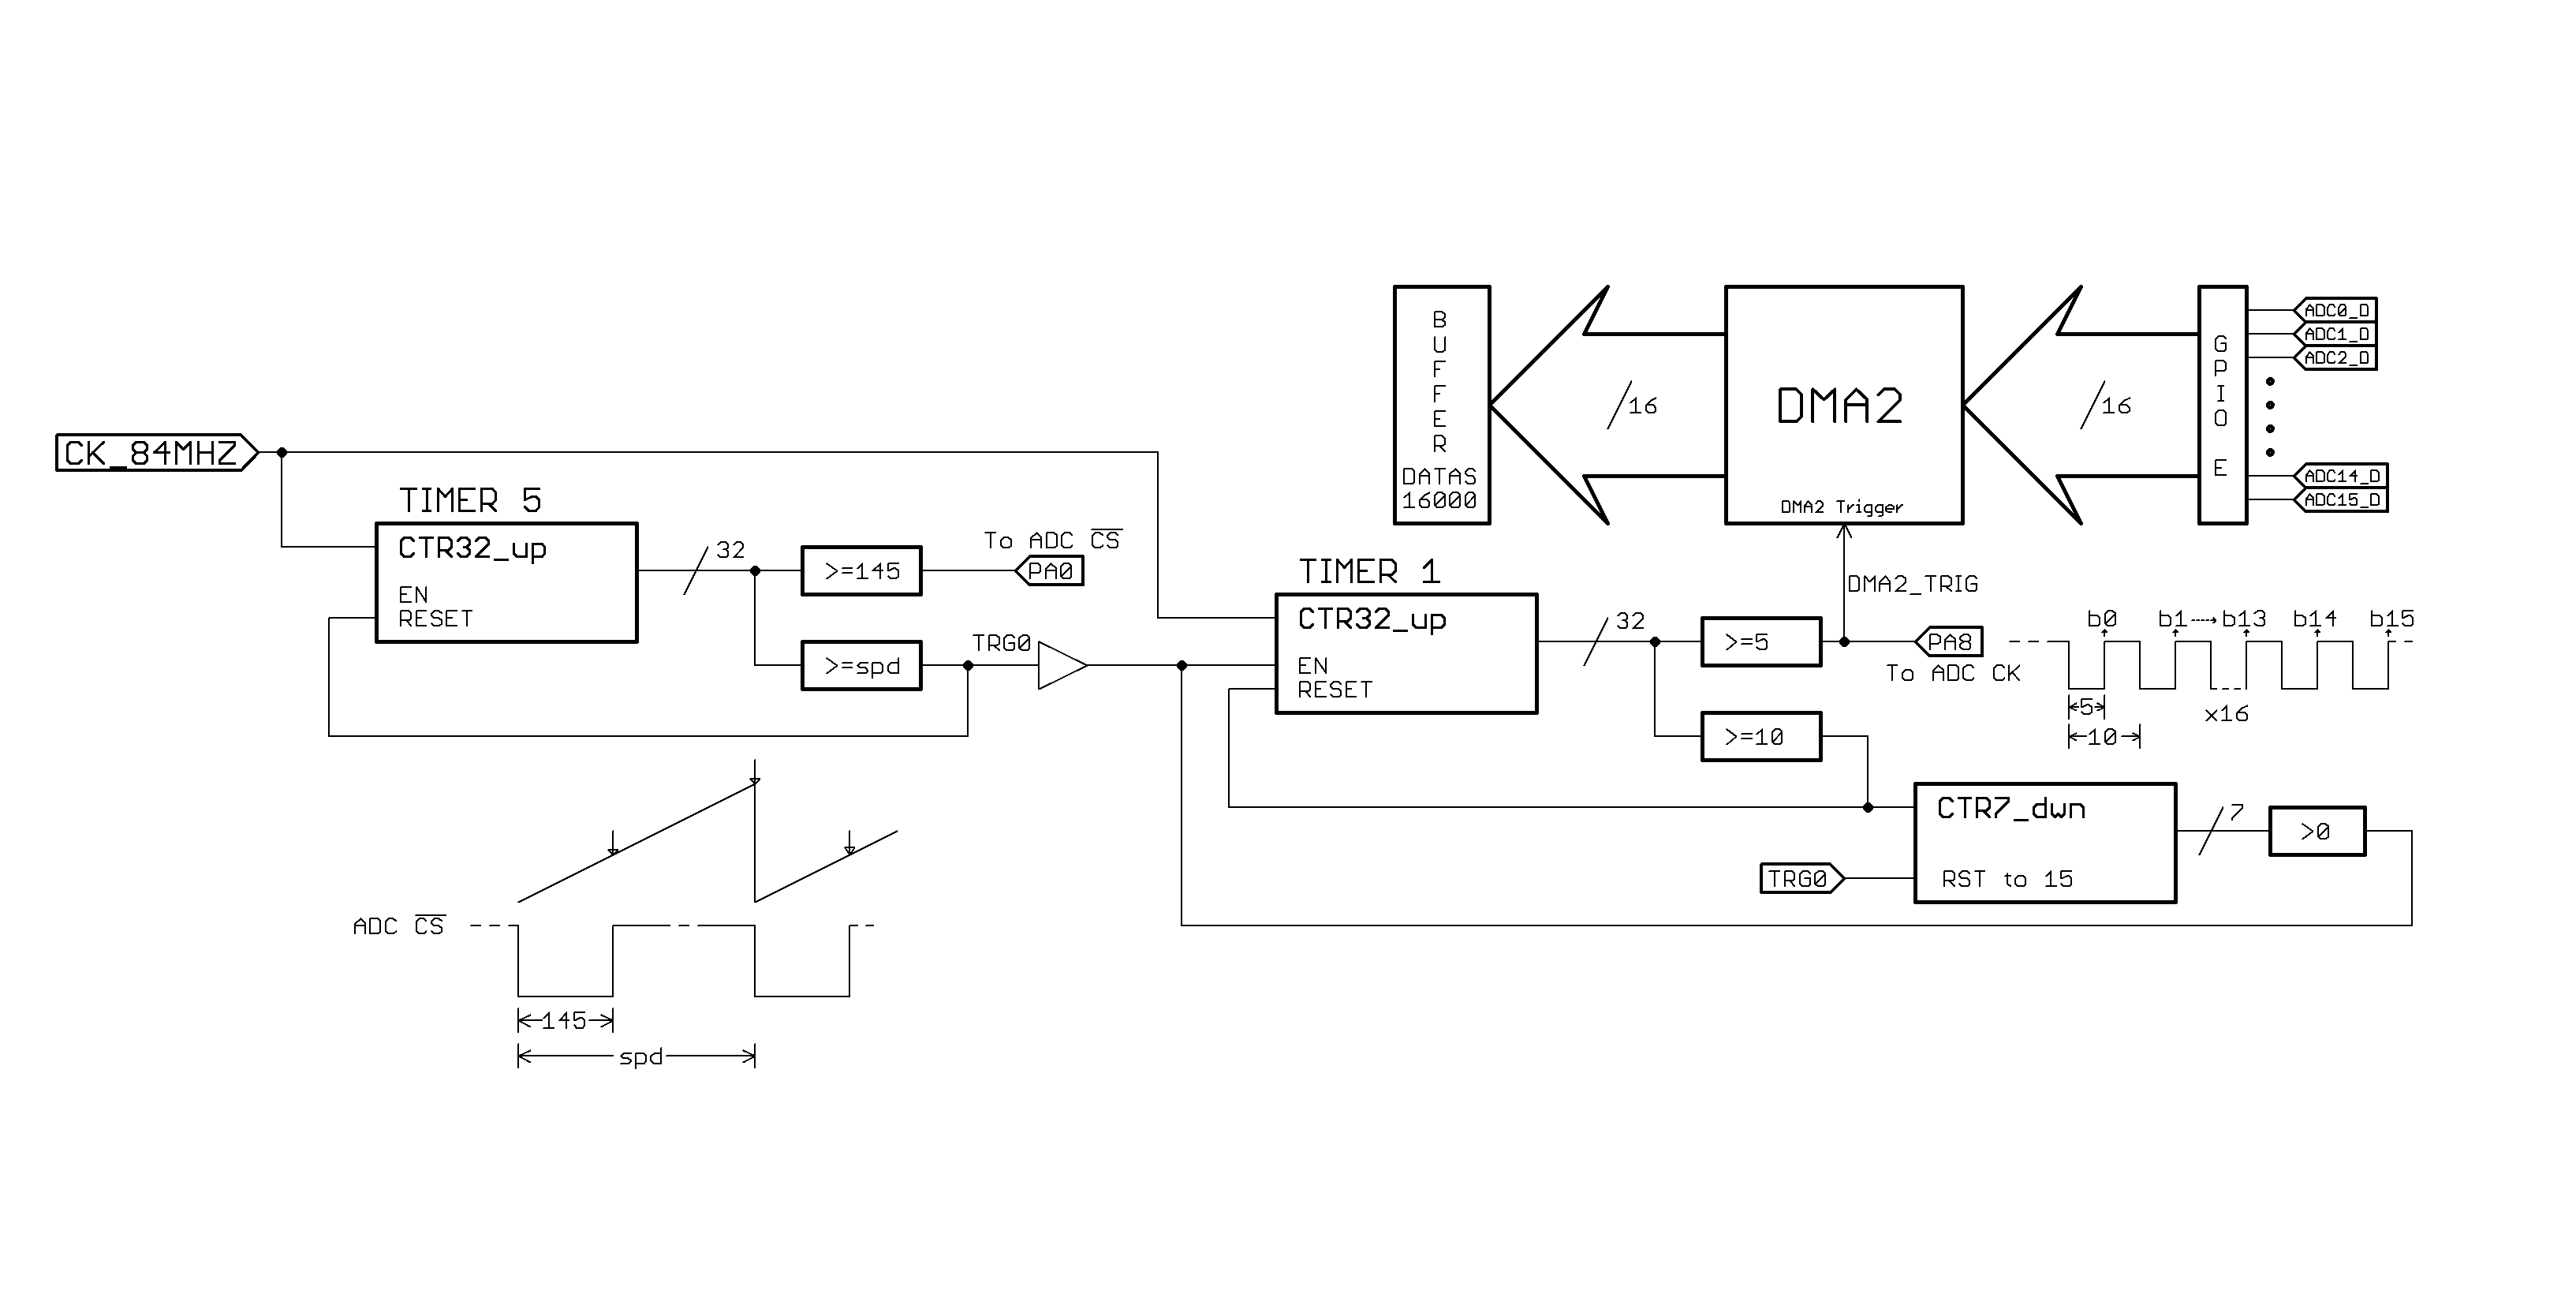
\includegraphics[width=1\textwidth]{../ADC.png}
      \caption{Full ADC Driver with DMA}
  \end{center}
\end{figure}


\subsection{ADC Timers}

Timer 5 drives the Chip Select lines.
It is configured as a 32-bit up-counting timer clocked at 84MHz, uses output compare unit 1 to control pin PA0 (connected to ADC $\overline{\mbox{\texttt{CS}}}$ ), and is set to run in continuous mode.
The ADC sampling frequency is controlled by the $\overline{\mbox{\texttt{CS}}}$ line, which is controlled by the period of Timer 5.
When a host computer requests an ADC trigger, it sends a sampling frequency along with it.
The appropriate $\overline{\mbox{\texttt{CS}}}$ period is calculated and assigned to the variable \texttt{spd} (sampling period).
Timer 5's output compare mode 1 is set to PWM2 mode, where PA0 is low when the counter is less than the compare value and high when the counter is greater than the compare value.
At update, Timer 5's count value is reset to 0, so PA0 falls to 0V and initiates a conversion.
When Timer 5 counts to 145, $1.7\mu S$ later, the conversion is complete and PA0 rises to 3.3V, until the count reaches \texttt{spd} and the cycle starts again.
Timer 5 is also configured in Master Mode and sends a trigger signal on TRG0 at each update event.
In this case, the signal on TRG0 is used to enable Timer 1.

\begin{figure}[H]
  \begin{center}
      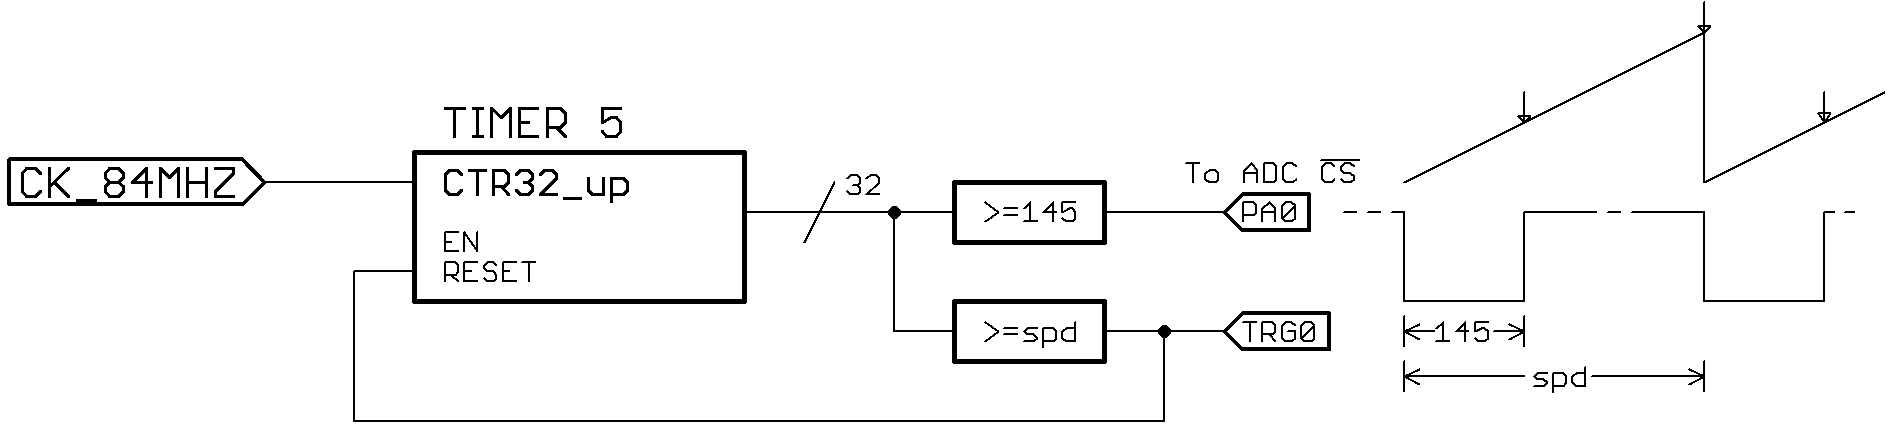
\includegraphics[width=1\textwidth]{../tim5.png}
      \caption{ADC Chip Select Timer}
  \end{center}
\end{figure}

Timer 1 drives the ADC Clock lines and behaves as a $1\mu S$ on - $1\mu S$ off 16-shot timer.
It's also configured as a 32-bit up-counting timer clocked at 84MHz, but it's only enabled by the TRG0 signal from Timer 5.
Like Timer 5, it uses output compare unit 1 to control an output pin, in this case \texttt{PA8}.
Unlike Timer 5, it's set to run in one-shot mode with a repetition counter that is preloaded with a value of 15.
The output compare unit is set to run in PWM2 mode with fixed compare and update registers.
When Timer 1 counts to 5, the compare unit fires and PA8 goes high.
When the count reaches 10, the timer is updated, PA8 goes low, and the repetition counter decrements.
The timer continues to run, toggling PA8 and decrementing the repetition counter, until the repetition counter reaches a value of 0.
Once the repetition counter reaches 0, the next Timer 1 update disables the timer.



\begin{figure}[h!]
  \begin{center}
      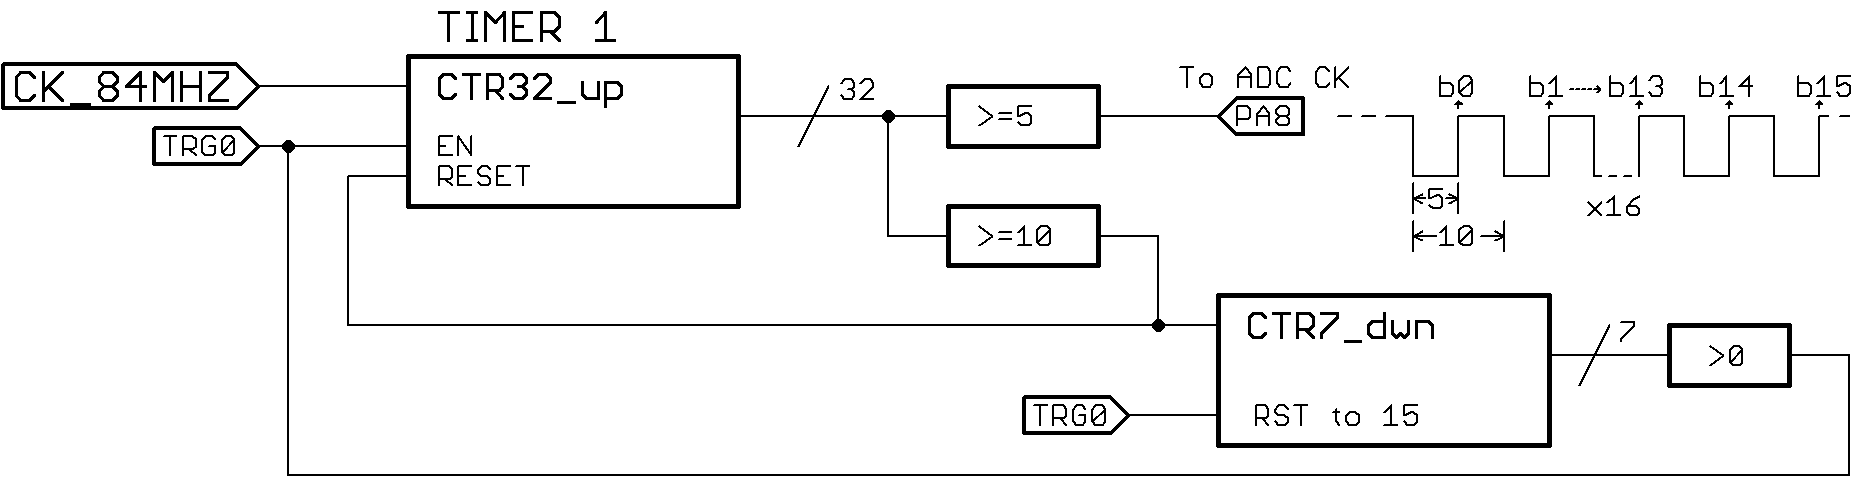
\includegraphics[width=1\textwidth]{../tim1.png}
      \caption{ADC Clock Timer}
  \end{center}
\end{figure}


\subsection{ADC DMA}

A DMA controller is used to store serial ADC data from up to 16 ADCs in parallel.
On each clock cycle, DMA2 takes the 16-bit integer value represented by the state of the 16 pins on \texttt{PORT E} and stores it in memory. 
As shown in Figure \ref{fig:adc-timing}, the ADC data pin is updated on a falling clock signal.
To record the state of the data pin, DMA2 is triggered to start a data transfer on every compare event from Timer 1, which corresponds with the rising edge of the clock signal.

\begin{figure}[H]
  \begin{center}
      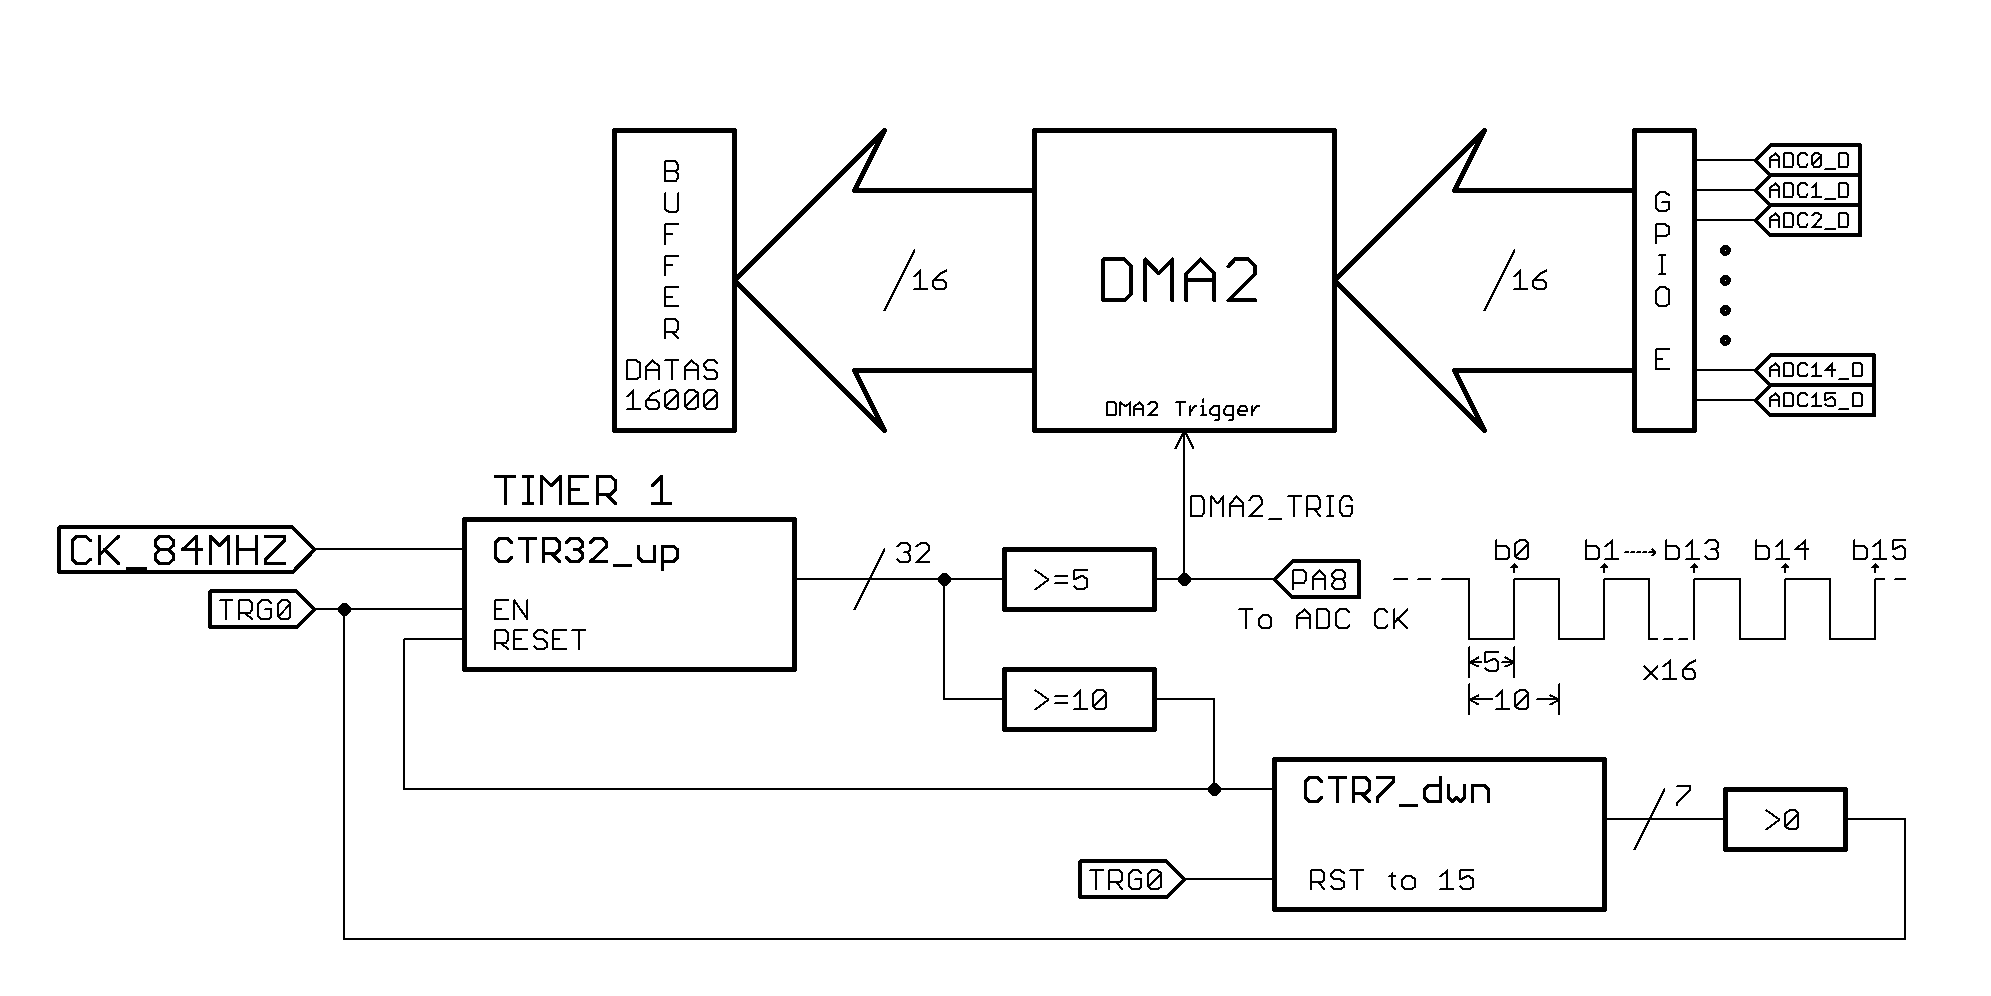
\includegraphics[width=1\textwidth]{../ADC-DMA.png}
      \caption{ADC Clock Timer Triggers DMA2}
  \end{center}
\end{figure}

When Timer 5 is enabled, DMA2's 'number of data' [to transfer] register is set to 16000  and the ADCs continuously sample at the sample period defined by \texttt{spd}.
In each cycle of Timer 5, Timer 1 toggles the clock line 16 times, triggering DMA2 on each rising edge.
With each DMA trigger, DMA2's number of data register decrements.
When the register reaches 0, an interrupt fires that disables Timer 5 and begins the data reconstruction process.


\subsection{Data Reconstruction}

Since the serial data stream from each ADC is stored sequentially, the actual A/D readings need to be reconstructed after they are recorded.
In Figure \ref{fig:data-reconstruct}, the binary data stored in \texttt{datas} is examined.
Each 16-bit integer in \texttt{datas} contains one bit of data from each of the 16 pins on \texttt{PORT E}, which connect to the data pins on the external A/D converters.
Here, each letter represents the data from a particular external ADC.

\begin{figure}[h]
\begin{center}
\begin{tabular}{ r|c c c c c c c c c | }
\multicolumn{1}{r}{Bit Index}
 &  \multicolumn{1}{c}{$b_{15}$}
 &  \multicolumn{1}{c}{$b_{14}$}
 &  \multicolumn{1}{c}{$b_{13}$}
 &  \multicolumn{1}{c}{$b_{12}$}
 &  \multicolumn{1}{c}{$...$}
 &  \multicolumn{1}{c}{$b_{3}$}
 &  \multicolumn{1}{c}{$b_{2}$}
 &  \multicolumn{1}{c}{$b_{1}$}
 &  \multicolumn{1}{c}{$b_{0}$}\\
\cline{2-10}
\texttt{datas[0]} 
 & $p_{15}$ & $o_{15}$ & $n_{15}$ & $m_{15}$ & ... & $d_{15}$ & $c_{15}$ & $b_{15}$ & $a_{15}$
  \\ \cline{2-10} \cline{2-10}
 \texttt{datas[1]} 
 & $p_{14}$ & $o_{14}$ & $n_{14}$ & $m_{14}$ & ... & $d_{14}$ & $c_{14}$ & $b_{14}$ & $a_{14}$
  \\  \cline{2-10} 
 \texttt{datas[2]} 
 & $p_{13}$ & $o_{13}$ & $n_{13}$ & $m_{13}$ & ... & $d_{13}$ & $c_{13}$ & $b_{13}$ & $a_{13}$
  \\  \cline{2-10} 
 \texttt{datas[3]} 
 & $p_{12}$ & $o_{12}$ & $n_{12}$ & $m_{12}$ & ... & $d_{12}$ & $c_{12}$ & $b_{12}$ & $a_{12}$
  \\  \cline{2-10} 
$\vdots$\hspace{2em}
 & $\vdots$ & $\vdots$ & $\vdots$ & $\vdots$ & ... & $\vdots$ & $\vdots$ & $\vdots$ & $\vdots$
  \\  \cline{2-10} 
 \texttt{datas[13]}
 & $p_{2}$ & $o_{2}$ & $n_{2}$ & $m_{2}$ & ... & $d_{2}$ & $c_{2}$ & $b_{2}$ & $a_{2}$
  \\  \cline{2-10} 
 \texttt{datas[14]}
 & $p_{1}$ & $o_{1}$ & $n_{1}$ & $m_{1}$ & ... & $d_{1}$ & $c_{1}$ & $b_{1}$ & $a_{1}$
  \\  \cline{2-10} 
 \texttt{datas[15]}
 & $p_{0}$ & $o_{0}$ & $n_{0}$ & $m_{0}$ & ... & $d_{0}$ & $c_{0}$ & $b_{0}$ & $a_{0}$
  \\  \cline{2-10} 
 \texttt{datas[16]}
 & $p_{15}$ & $o_{15}$ & $n_{15}$ & $m_{15}$ & ... & $d_{15}$ & $c_{15}$ & $b_{15}$ & $a_{15}$
  \\  \cline{2-10} 
  
\end{tabular}
\end{center}
\caption{\texttt{datas[0:16]}}
\label{fig:data-reconstruct}
\end{figure}

To reconstruct the data collected from ADC$_a$[0], a routine iterates through \texttt{datas[0:15]}, summing appropriately bit-shifted $b_0$'s.\\
ADC$_a$[0] = ($a_{15}<<15)+(a_{14}<<14)+(a_{13}<<13)+...+(a_{2}<<2)+(a_{1}<<1)+a_0$\\
To reconstruct all of the waveform recorded, the routine iterates through \texttt{datas[0:16000]}, reconstructing 1000 samples from each ADC.

After reconstruction, the data is sent to a host program over USB for further processing.

\section{DAC}

The STM32F407's onboard DAC is used as a signal source for impedance testing.
The DAC is configured to update on a timer, and is fed new waveform values from a wavetable by DMA1.

\begin{figure}[H]
  \begin{center}
      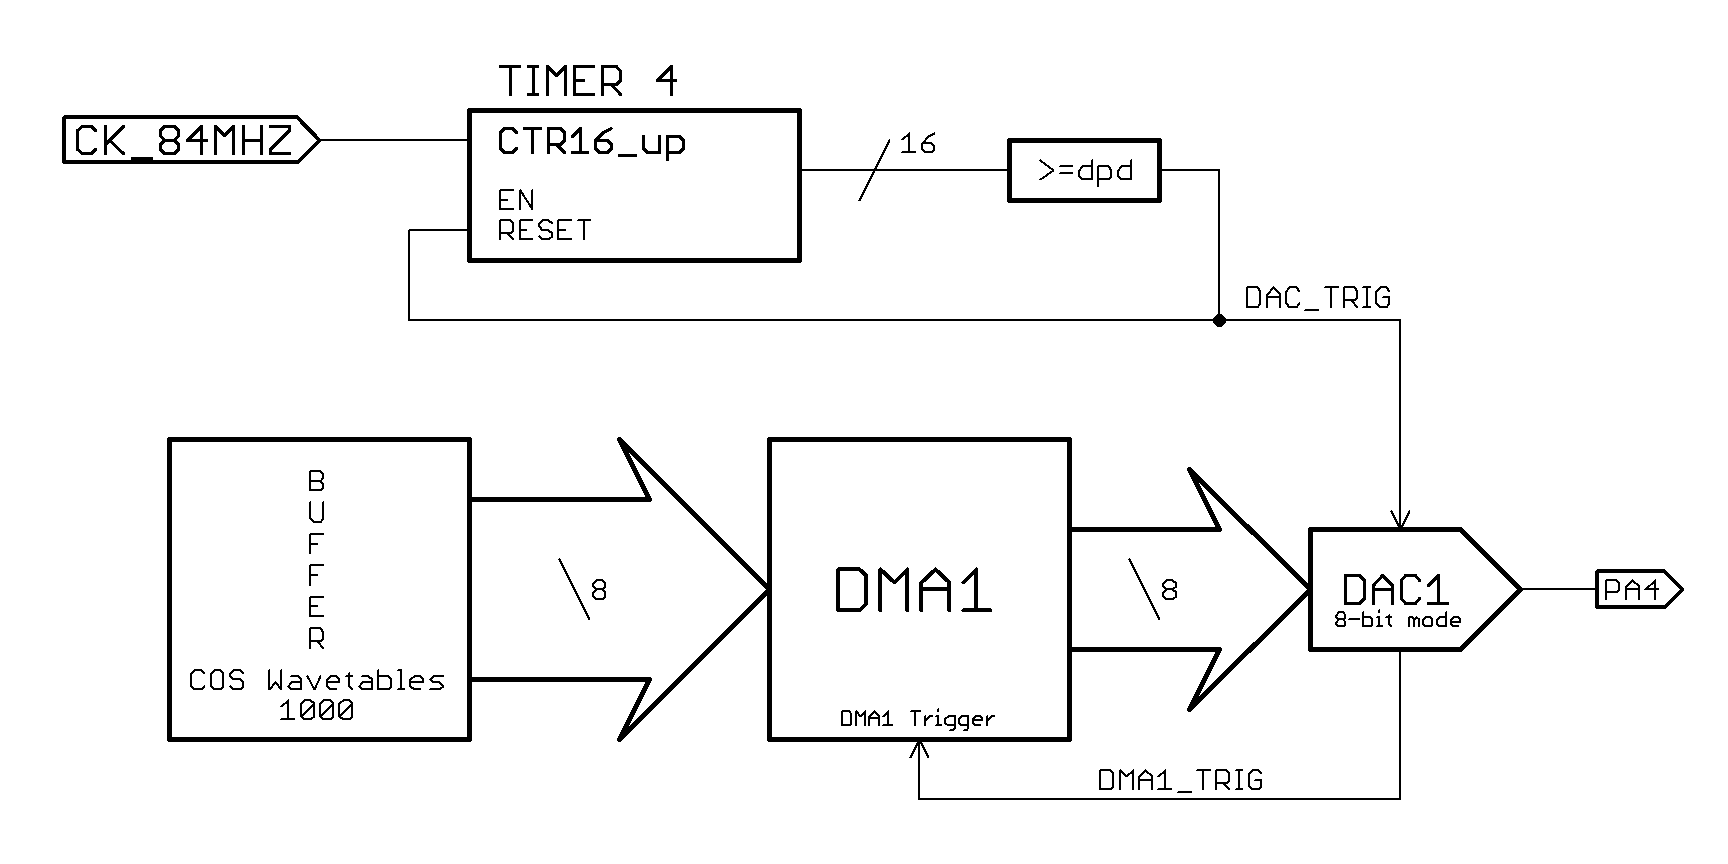
\includegraphics[width=1\textwidth]{../DAC-DMA.png}
      \caption{DAC Timer Triggers DMA1}
  \end{center}
\end{figure}


Timer 4 is configured as a 16-bit up-counting timer with period \texttt{dpd}, set by command over USB.
On update, Timer 4 is a master to DAC1, and triggers the DAC to output a new value.
The DAC, in turn, triggers a data transfer from DMA1, which transfers the next value in the cosine wavetable to DAC1.


\subsection{DAC Wavetables}

There are three DAC wavetables, each 1000 bytes long.
The first wavetable has four cycles of cosine, the second has 10, and the last has 40.
The different-sized wavetables are necessary to maintain high-fidelity output signals at low frequency while still permitting high-frequency output.

\section{USB}


\subsection{USBACM}


\subsection{Command List}
%\end{document}